\chapter{Case Study Design} \label{methods}
This study will use the \textit{Holystic Exploratory Case Study} research methodology as described by \cite{case_study_guide}. Furthermore, I will follow the guidelines expressed by Runeson and H{\"o}st \cite{case_study_software_engineering} that specifically target the Software Engineering field. Moreover, they provide a Checklist that I extensively used while performing the study.

\todo{Mention Checklist in the appendix with links on where is possible to find the answers.}


%
%
% START CASE DESCRIPTION
%
%
\section{Case Definition}	\label{case-description}
For properly characterize the Case under study \cite{case_study_guide} suggest to describe three items. Namely 1) the context in which the Case is, 2) the Case itself, and 3) the Units of Analysis used during the study.

This study took place in the Swedish office of the Company, which globally employes more than 3000 people scattered in several offices. Its core business is licensing software products for mangaing personnel and equipments in the context of Transportation. The portfolio offers differnet solutions to cover sevaral business needs in terms of short or long term planning, personnel optimization etc.

Internally, teams use Scrum for managing their development activities. They have great freedom in chosing sprint length, and the Definition of Done, which is build on top of a minimum one provided by the company. Teams are cross functional, meaning that they contain people with different areas of expertise and are self-contained meaning that they should carry out all software related activities indipendently.

This last fact is important for this study. In fact, all testing activities are carried on indipendently, following the minimum guidelines expressed in the Definition of Done. However, this lenient artifact causes teams to use different testing strategies for complying with testing pipeline. 

As shown in Fig. \ref{fig:testing_pipeline} this pipeline is composed of four main levels (lower to higher): unit tests, components tests, system tests, end to end tests. These mentioned level do not differentiate between functional and quality (non-functional) testing types as these can take place at any level. 

Unit tests are carried on by developers alongside development activities and aim to test the System at function / class level. Therefore, there is a high number of those tests, which tend to be fast to execute and simple. Developers follow almost the same guidelines specified for the actual code, with the sole exception that, according to the minimum definition of done, they are not reviewed.

Component tests target interaction between macro software-entities and aim to ensure that the sub-parts of the system deliver the desired functionalities. What is tested at this level is the exposed APIs entry points and not the internal mechanics of the source code.

System tests are executed to assure that user functionalities and business processes of a single system behaves according to specification. These tests are executed at user interface level with realistic data sets and possibly data volume. Furthermore, the system is an exact copy of production environmets. End to End tests are similar in concept and execution to System tests, but they test the interaction of two or more complete systems.

\todo{Improve figure \ref{fig:testing_pipeline} readibility}
\todo{Extract the image from the testing chapter document}

\begin{figure}[ht]
    \centering
    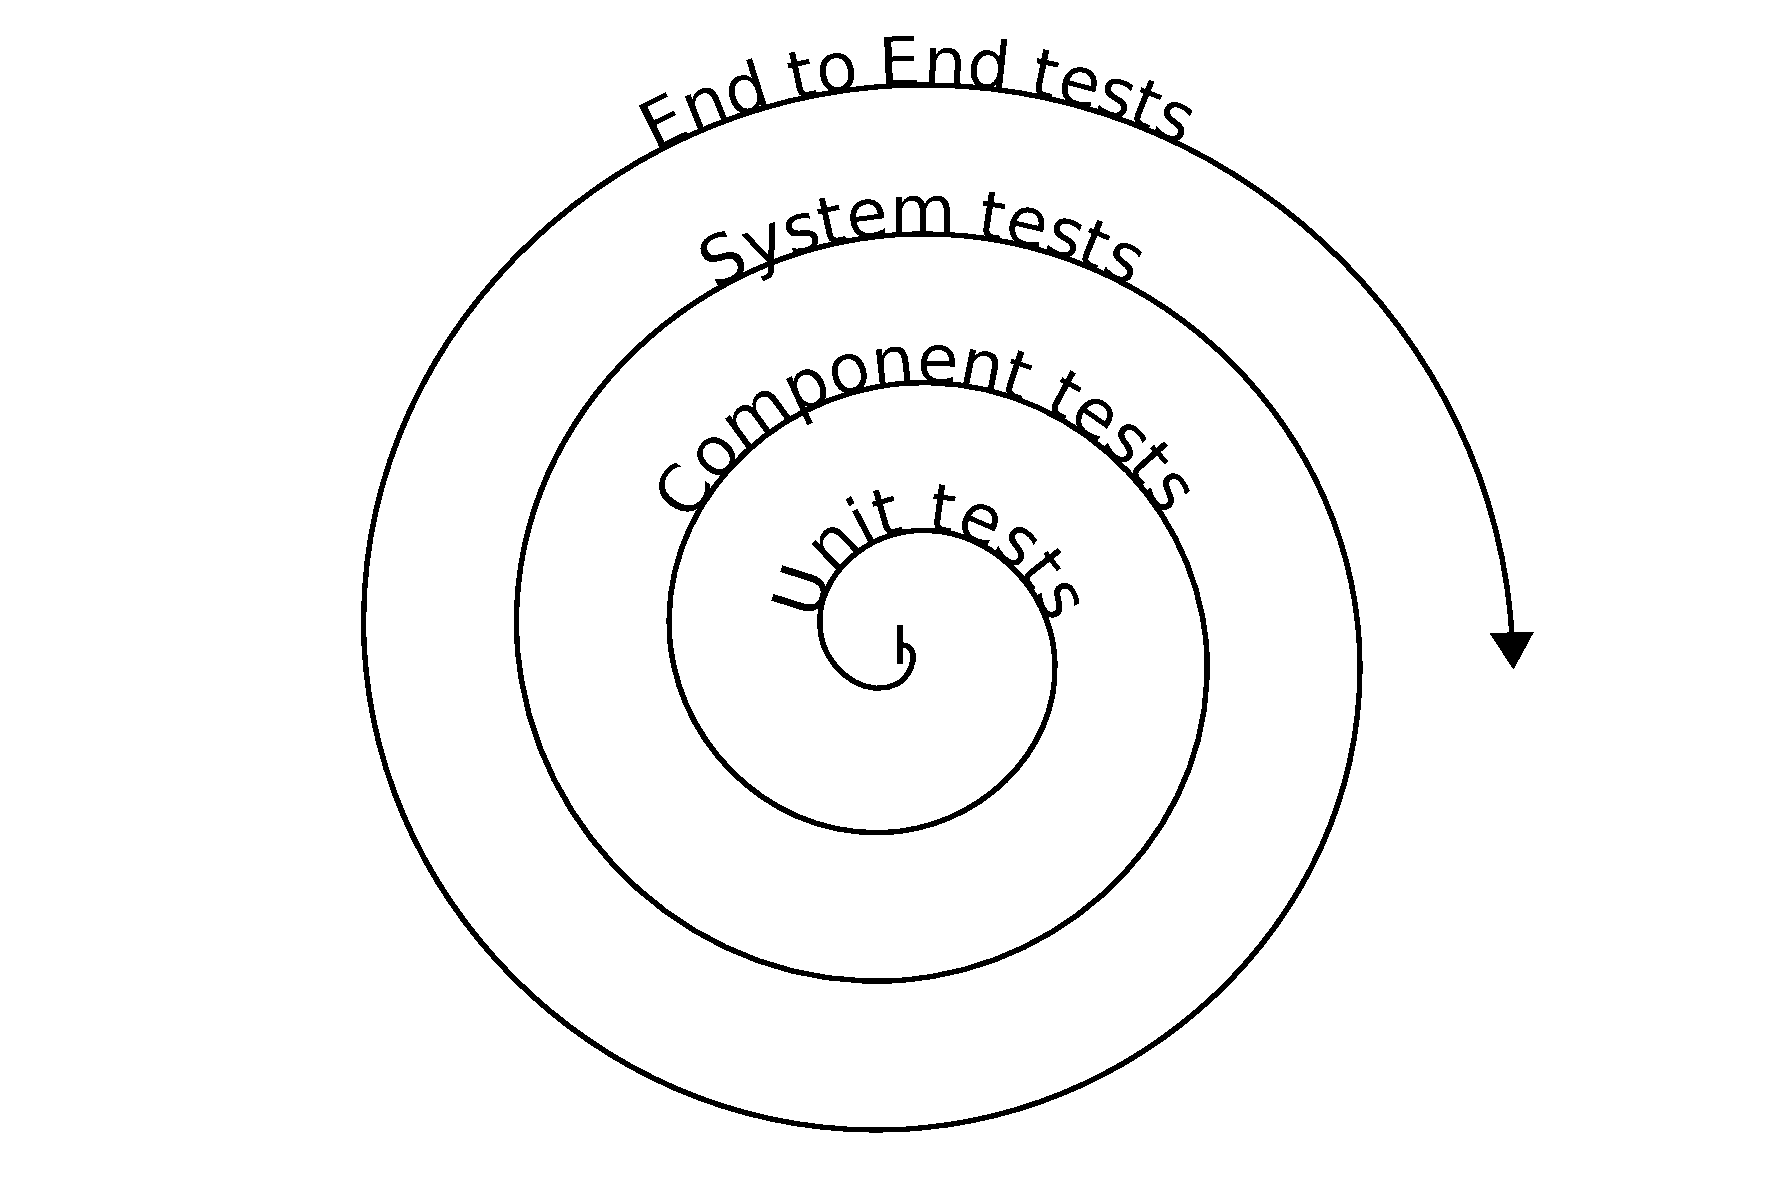
\includegraphics[width=\textwidth]{figure/testing_pipeline.pdf}
    \caption{Testing pipeline in use at the Company}
    \label{fig:testing_pipeline}
\end{figure}

For narrowing the scope to a manageable size I decided to use as \textit{Cases} the projects that use Hewlett Packard UFT (Unified Functional Test) for GUI testing (formerly known as QTP). It has been introduced one year ago (Q3 2014) and allow testers to mix Property Based GUI testing (2nd generation tool) and Image Recognition GUI testing (3rd generation). Within these projects I will evaluate the maintenance activities that target the two higher testing levels of the functional part of the mentioned pipeline. Specifically how much extra maintenance derives from the use of bad code practices used in GUI test scripts. With that said, the chosen \textit{Unit of Analysis} are the such maintenance activities. 
    

%
%
% END CASE DESCRITPION
%
%

%
%
% START DATA GATHERING
%
%
\section{Data Gathering}
As recommended by Yin \cite{case_study_guide,case_study_software_engineering}, I gathered data from various sources in order to increase Data Triangulation and hence improve the study's reliability. Precisely, the sources used are: 1) Informal Interviews (a.k.a.\ Coffe Machine / Water Bowl Interviews), 2) Mining of Comapany's Forum, 3) Mining of Comapny's Issue Tracker, 4) Mining of Repositories, and 5) Semi-structured Interviews.

However, some of the data sources were used as secondary sources, meaning that they assited the inquiry conducted by other methods. I.e.\ I used Informal Interviews, and the mining of the forum mainly during the first phase of this Exploratory Case Study for narrowing the scope. Consequently, I achieved a more focused analysis of other sources (e.g.\ Analysis of the repositories).

Finally, considering the extensive amount of data that has been generated, I won't directly include it in this Report. Instead, it is available online at \href{http://somthing/}. However, readers should be aware that the raw Data was anonymized and every sensitive information was also removed. 

\todo{Insert link to thesis database}
\todo{Mention that data is 3rd stage}
\todo{Mention that I used both quantitative and qualitative sources for improving reliability}

\subsection{Informal Interviews}
I used this Data Source to overcome resource's scarcity. In fact, I had to limit the number of Formal Interviews (see \ref{semi-structured_interviews}) and hence I opted for this source. However, considering their non-reproducible nature I decided to not use them for sensitive parts of the study like Theory Validation. \tocite{Reference a peper on such interviews}

The method used for each one of these Interviews varied depending of several factors. Firstly, the frequency of such Interviews was random. They occurred during lunch and/or coffee breaks. The settings also varied both in terms of interviewee and location. However, most of them occurred in the coffee room that the company provides to its employees. Furthermore, the topic covered depended on my current insight. In fact, they helped me formulate a theory draft in a \textit{trial and error} fashion. For instance, at the beginning my questions were about documentation and similar artifacts. Afterwards the scope narrowed with questions targeting current problems and solutions related to test maintenance. These last questions allowed me to discover critical time frames that were also reflected in the Company's Repositories.

As a final note, due to the randomness of both subjects, locations, and frequency, I was unable to create proper artifacts for these interviews. However, the Thesis Database contains brief descriptions of the topics covered by each one of these.

\subsection{Mining of The Forum} \label{mining_forum}
In order to enable Knowledge Sharing the company deployed a Collaborative Software / Fourm. The one in use is Confluence, developed and maintained by Atlassian. In it both Technical and Non-Technical Employers create pages for sharing procedures, ideas, or create non synchronous discussion threads about problems. For these reasons this source is valuable since it contains numerous informations, which can shed light on the problems this Thesis aim to study.

However, considering the magnitude of the data included I decided to follow a systematic approach in order to ensure that no relevant information was missed. In fact, the system contains data covering several years and include several thousands discussions threads and many more answers. To overcome this probelm I used the embedded search enginge. The Strings entered were included withing double quotes in order to enable the exact match feature. This choice was needed to limit the number of results. For instance, \textit{test maintenance} yielded 8467 results whereas \textit{"test maintenance"} 28. Furthermore, this reduced result set has gone through two filtering steps before being included.

The first coarser filter is based on a reduced time frame. I eliminated hits older than 1 year for several reasons. Firstly, the Testware stack has been cahnged during last year (2014) and hence my findings could be biased by information not relevant or dependant to the old technologies. Secondly, wehn deciding an adequate time span I considered the mortality of the resources. In fact, the Company greatly relies on consultants and their turnover is shorter than normal employees.

The second finer filter is based on the relevance. In fact, the mentioned search engine uses a full-text search and hence results are returned even if someone commented the original post mentioning the considere keywords. Therefore, I decided to eliminate every hit that did't contain the keywords in the title or in the body of the original post. However, if the answers mentioning the keyword were referring to another entry/issue or esplicitly introducing the topic summarized by the keyword I included them.

Finally, the remaining set of posts has been carefully read and pertinent ones has been anonymized and transcribed in the Thesis database. Table \ref{tab:confluenceMiningResults} the results obtained for each step for the keywords used.

\begin{table}[htb]
	\centering
	%\renewcommand{\arraystretch}{1.2}
	\caption{Number of hits in Confluence for a given keyword}
	\label{tab:confluenceMiningResults}
	\begin{tabulary}{\textwidth}{|L|L|L|L|}
		\hline
		\textbf{Keyword} & 
		\textbf{Total hits} &
		\textbf{After First Filter} &
		\textbf{After Second Filter}\\ \hline
		
		\textit{"test mainteneance"} &
		28 &
		18 &
		9 \\ \hline
		
		\textit{"tests strategy"} &
		297 &
		138 &
		11 \\ \hline
		
		\textit{"test refactoring"} &
		13 &
		3 &
		3 \\ \hline
		
		\textit{"test quality"} &
		36 &
		4 &
		4 \\ \hline
		

	\end{tabulary}		
\end{table}

\subsection{Mining of The Issue Tracker / Backlogs}

The Company uses an all in one solution for managing issues and their Agile Environments: JIRA + Agile Plugin. These solutions are also managed by Atlassian. Given the vastitiy of items in the database the assumptions I made for the Confluence Forum still apply. Furthermore, also the filtering procedure is similar. However, I attributed more importance to this source.

In fact, both issues and User Stories are one of the aforementioned maintenance triggering factors. Furthermore, it is possible to track such items to specific commits included in the repositories. Therefore, this source allows a high degree of traceability and it can be used to consolidate some of my insights.

The filtering process differs due to the different data formats used by reporting User Stories and Issues. In fact, it is more concise and hence the probability of a hit by keyword is lower. Therefore I decided to include in my search the related issues of each result in order to compensate.

However, due to the highly sensitive informations about issues, bugs, and planned features included in this source I cannot disclose any part of them and hence I limit to report the the keywords used with the raw numbers.

\todo{Make table/chart/appendix with links between issues related to testing and repositories commits}

\begin{table}[htb]
	\centering
	%\renewcommand{\arraystretch}{1.2}
	\caption{Number of hits in JIRA for a given keyword}
	\label{tab:jiraMiningResults}
	\begin{tabulary}{\textwidth}{|L|L|L|L|}
		\hline
		\textbf{Keyword} & 
		\textbf{Total hits} &
		\textbf{After First Filter} &
		\textbf{After Second Filter}\\ \hline
		
		\textit{"test mainteneance"} &
		28 &
		18 &
		9 \\ \hline
		
		\textit{"tests strategy"} &
		297 &
		138 &
		11 \\ \hline
		
		\textit{"test refactoring"} &
		13 &
		3 &
		3 \\ \hline
		
		\textit{"test quality"} &
		36 &
		4 &
		4 \\ \hline
		

	\end{tabulary}		
\end{table}

\todo{Fix table with data when I will have it}


\subsection{Analysis of The Repositories} \label{analysis_of_the_repos}
The company extensively uses \textit{Concurrent Versions System}. At the time of writing their system contains 870 repositories of various size belonging to 20 projects. Some of them, however, are cross project. They also have deployed two different tools to browse such repositories with ease: \textit{HgWeb} and \textit{Crucible + FishEye}. They are migrating to the second one since it also allows asynchronous code reviews and is can be integrated with the Issue Tracker and the Forum.

Given the amount of data contained in this archivial source, I used data coming from other sources to select the subset of repositories that better suites the goal of this Thesis. I.e.\ a selected number of repositories targeting test code that are currently under active development or maintenance. In addition, the Issue Tracker analisys combined with the informal interviews allowed me to constrain the mining activities to specific time frames that are of particular interest for maintenance activities. 

\todo{Finishing this section describing what I did with the commits when I will actually perfom the mining}

\subsection{Semi-Structured Interviews} \label{semi-structured_interviews}
During this study I conducted a total of \inote{Number of Interviews here} interviews following the guidelines expressed in \cite{interview_guideline}. I opted for the semi-structured format in order to have enough flexibility to adapt my inquiry while maintaining the scope constrained.

The purpose of this data source was two-fold: to provide me some insights during the first phase of the study, and to validate my findings during the final stage of it. For the first purpose I conducted one interview to get up to speed with the system faster and also to start generating some ideas about the Testing situation within the Company. The second one, instead, used the remaining interviews and helped me confirming my findings and create some open questions that might be useful for future studies on the topic.

\todo{Finish the subsection describing settings, who has been interviewed and such
}



%
%
% END DATA GATHERING
%
%


%
%
% START DATA INTERPRETATION
%
%
\section{Interpretation of the Data} \label{data_interpretation}

